% !TeX program = xelatex
\documentclass{beamer}
\usepackage{xeCJK}
\usepackage{bookmark}
% 图片路径
\graphicspath{{Figures/}}
% 设置主题
\usetheme{Berkeley}
\usecolortheme{beaver}
\setbeamercolor{title in sidebar}{fg=black}
\setbeamercolor{section in sidebar shaded}{fg=black}
\usefonttheme{serif}
% 报告基本信息
\logo{\includegraphics[height=0.09\textwidth]{whulogo.eps}}
\title[Graph Embedding]{图表示学习}
\author[S. Zhou]{Zhou Shen}
\institute{School of Computer Science, Wuhan University}
\date{\today}

\begin{document}
% -----------------------------------------首页-----------------------------------------
\begin{frame}
    \titlepage
\end{frame}
% ----------------------------------------目录页----------------------------------------
\begin{frame}{Outline}
    \tableofcontents
\end{frame}
% ---------------------------------------Word2Vec---------------------------------------
\section{Word2Vec}
% one-hot encoding
\begin{frame}{Word2Vec}
    \framesubtitle{One-Hot Encoding}
    \centering\includegraphics[height=5cm]{one_hot.png}
\end{frame}
% one-word context
\begin{frame}{Word2Vec}
    \framesubtitle{One-Word Context}
    \centering\includegraphics[height=4cm]{word2vec_1.pdf}
    \begin{equation}
        \mathbf{h}=\mathbf{W}^{T} \mathbf{x}=\mathbf{W}_{(k, \cdot)}^{T}:=\mathbf{v}_{w_{I}}^{T}, u_j=\mathbf{v}_{w_j}^{\prime}h
    \end{equation}
    \begin{equation}
        p\left(w_{j} \mid w_{I}\right)=y_{j}=\frac{\exp \left(u_{j}\right)}{\sum_{j^{\prime}=1}^{V} \exp \left(u_{j^{\prime}}\right)}
    \end{equation}
\end{frame}
% Objective Function
\begin{frame}{Word2Vec}
    \framesubtitle{Objective Function}
    \begin{equation}
        \begin{aligned}
        \max p\left(w_{O} \mid w_{I}\right) &=\max y_{j^{*}} \\
        &=\max \log y_{j^{*}} \\
        &=u_{j^{*}}-\log \sum_{j^{\prime}=1}^{V} \exp \left(u_{j^{\prime}}\right):=-E
        \end{aligned}
    \end{equation}
    \begin{alertblock}{常用变形}
        $\min E=-u_{j^{*}}+\log \sum_{j^{\prime}=1}^{V} \exp \left(u_{j^{\prime}}\right)$
    \end{alertblock}
\end{frame}
% CBOW
\begin{frame}{Word2Vec}
    \framesubtitle{CBOW}
    \begin{columns}
        % 第一列
        \begin{column}{0.4\textwidth}
            \centering\includegraphics[height=6cm]{word2vec_2.pdf}
        \end{column}
        % 第二列
        \begin{column}{0.6\textwidth}
            $$\mathbf{h} = \frac{1}{C}(\mathbf{v}_{w_1} + \mathbf{v}_{w_2} + \cdots + \mathbf{v}_{w_C})^T$$
            $$
            \begin{aligned}
                E &=-\log p\left(w_{O} \mid w_{I, 1}, \cdots, w_{I, C}\right) \\
                &=-u_{j^{*}}+\log \sum_{j^{\prime}=1}^{V} \exp \left(u_{j^{\prime}}\right) \\
            \end{aligned}
            $$
        \end{column}
    \end{columns}
\end{frame}
% Skip-Gram
\begin{frame}{Word2Vec}
    \framesubtitle{Skip-Gram}
    \begin{columns}
        % 第一列
        \begin{column}{0.4\textwidth}
            \centering\includegraphics[height=6cm]{word2vec_3.pdf}
        \end{column}
        % 第二列
        \begin{column}{0.6\textwidth}
            $$
            \begin{aligned}
            E &=-\log p\left(w_{O, 1}, w_{O, 2}, \cdots, w_{O, C} \mid w_{I}\right) \\
            &=-\log \prod_{c=1}^{C} \frac{\exp \left(u_{c, j_{c}^{*}}\right)}{\sum_{j^{\prime}=1}^{V} \exp \left(u_{j^{\prime}}\right)} \\
            &=-\sum_{c=1}^{C} u_{j_{c}^{*}}+C \cdot \log \sum_{j^{\prime}=1}^{V} \exp \left(u_{j^{\prime}}\right)
            \end{aligned}
            $$
        \end{column}
    \end{columns}
\end{frame}
% Hierarchical Softmax
\begin{frame}{Word2Vec}
    \framesubtitle{Hierarchical Softmax}
    \centering\includegraphics[height=4cm]{word2vec_4.pdf}
    $$
        p\left(w=w_{O}\right)=\prod_{j=1}^{L(w)-1} \sigma\left([ n(w, j+1)=\operatorname{ch}(n(w, j)) ] \cdot \mathbf{v}_{n(w, j)}^{\prime}{ }^{T} \mathbf{h}\right)
    $$
\end{frame}
% Negative Sample
\begin{frame}{Word2Vec}
    \framesubtitle{Negative Sample}
    1. 词频计算
    $$
        weight(w_i) = \frac{count(w_i)^{0.75}}{\sum_{j}^{V} count(w_j)^{0.75}}
    $$
    2. 目标函数
    $$
        E=-\log \sigma\left(\mathbf{v}_{w_{O}}^{\prime}{ }^{T} \mathbf{h}\right)-\sum_{w_{j} \in \mathcal{W}_{\mathrm{neg}}} \log \sigma\left(-\mathbf{v}_{w_{j}}^{\prime}{ }^{T} \mathbf{h}\right)
    $$
\end{frame}
% ---------------------------------------DeepWalk---------------------------------------
\section{DeepWalk}
% 问题定义
\begin{frame}{DeepWalk}
    \centering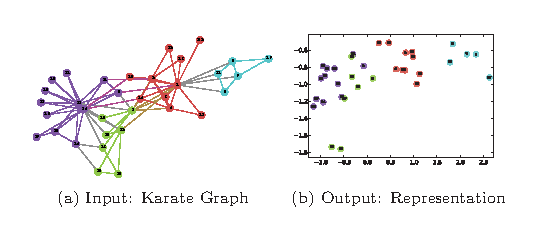
\includegraphics[height=3.8cm]{DeepWalk_1.eps}
    \begin{definition}{Problem Definition}
        Let $G = \left( V ,E \right)$, where $V$ are the members of the network, and $E$ be its edgs.
        Our goal is to learn $X_E\in \mathcal{R} ^{|V|\times d}$, where $d$ is number of 
        latent dimensions.
    \end{definition}
\end{frame}
% 为什么可以套用Word2Vec的思想
\begin{frame}{DeepWalk}
    \centering\includegraphics[height=4cm]{DeepWalk_2.pdf}
    \begin{alertblock}{Connection}
        The power-law distribution of vertices appearing in the short random walks follows 
        a power-law, much like the distribution of words in natural language.
    \end{alertblock}
\end{frame}
% 公式推导
\begin{frame}{DeepWalk}
    \begin{enumerate}
        \item give a sequence of random walk from vertice $i$
            \begin{equation}
                \mathcal{W}_{i}^{n}  = \{v_1, v_2, v_3, \cdots , v_n\}
            \end{equation}
        \item maximize the likehood
            \begin{equation}
                \operatorname{Pr}\left(v_i \mid \left(\Phi(v_1), \Phi(v_2), \cdots, \Phi(v_{i-1}))\right)\right)
            \end{equation}
            \begin{block}{Mapping Function $\Phi$}
                $\Phi: v \in V \longmapsto \mathcal{R}^{|V|\times d}$
                where $d$ is the number of dimensions                
            \end{block}
    \end{enumerate}
\end{frame}
% 为什么使用Skip-Gram
\begin{frame}{DeepWalk}
    \framesubtitle{Disadvantages and Optimizations}
    \begin{itemize}
        \item As the walk length grows, computing this objective function becomes unfeasible.
        \item Restricts the order in which vertices appear
    \end{itemize}
    \centering\includegraphics[height=3.1cm]{DeepWalk_3.pdf}
\end{frame}
% 优化目标与算法
\begin{frame}{DeepWalk}
    \framesubtitle{Algorithm}
    \centering\includegraphics[height=5cm, width=7cm]{DeepWalk_4.pdf}
    \begin{corollary}
        $\underset{\Phi}{\operatorname{minimize}}-\log \operatorname{Pr}\left(\left\{v_{i-w}, \cdots, v_{i-1}, v_{i+1}, \cdots, v_{i+w}\right\} \mid \Phi\left(v_{i}\right)\right)$
    \end{corollary}
\end{frame}
% ---------------------------------------Node2Vec---------------------------------------
\section{Node2Vec}
\begin{frame}{Node2Vec}
    
\end{frame}
% ---------------------------------------Stuc2Vec---------------------------------------
\section{Struc2Vec}
\begin{frame}{Struc2Vec}
    
\end{frame}
% ---------------------------------------LINE--------------------------------------------
\section{LINE}
\begin{frame}{LINE}
    
\end{frame}
% -----------------------------------------SDNE-----------------------------------------
\section{SDNE}
\begin{frame}{SDNE}
    
\end{frame}
% -----------------------------------------END------------------------------------------
\end{document}